\documentclass{ximera} 


% vier voorkeuren die je meteen zelf kan instellen:
\def\uitbr{0} % waarde 1 als je Uitbreiding in de marge wilt, 0 als je dat niet wilt 
\def\wsg{0} % waarde 1 als je verwijzingen naar Wiskunde Samen gevat² in de marge wilt, 0 als je dat niet wilt
\def\rectoverso{0} % waarde 1 als je het PDF-bestand recto-verso wilt laten afdrukken, 0 als je het recto wilt
\def\voetn{1} % waarde 1 als je de voetnoten wilt, 0 als je dat niet wilt 

% marges:
\usepackage[paper=a4paper,margin=3.4cm,marginparwidth=2cm]{geometry}

% packages algemeen:
\pdfOnly{
\usepackage[english,dutch]{babel}
}
\usepackage{amsfonts}
\usepackage{amsmath} %  o.a. \eqref en \text, omgeving equation*
\usepackage{amssymb} % o.a. \nmid
\usepackage{amsthm} % o.a. omgeving proof
\usepackage{graphicx} % o.a. figuren
\usepackage{xcolor} % \color
\usepackage[disable]{todonotes} % \todo 
\usepackage{comment} % omgeving comment
\usepackage{xcolor} % kleuren 
\usepackage[skip=7pt plus1pt, indent=0pt]{parskip} % skip = verticale ruimte tussen twee alinea's, indent = insprong bij nieuwe alinea
\usepackage{multicol} % kolommen
\usepackage{xfrac} % breuken

\usepackage{siunitx} % SI eenheden
\usepackage{eso-pic} % achtergrond voorpagina
\usepackage{tabularx} % kolommen voor rekenmachine
\usepackage{rotating} % voor omgeving turn

% voor figuren met PSTricks:
\usepackage{pstricks} 
\usepackage{pstricks-add}
\usepackage{pst-plot}
\usepackage{pst-node}
\usepackage{pst-coil}
\usepackage{auto-pst-pdf}

% voor figuren met TikZ:
\usepackage{tikz} 
\usepackage{tkz-euclide} 
\usepackage{pgfplots} 
\usetikzlibrary{calc,intersections,through,backgrounds,patterns} 
\pgfplotsset{compat=newest}
\usepgfplotslibrary{fillbetween,colormaps}
\usepackage{import}
\usepackage{tikz-3dplot}

% zelfde parskip in minipage:
\makeatletter
\setlength{\parskip}{\medskipamount}
\newcommand{\@minipagerestore}{\setlength{\parskip}{\medskipamount}}
\makeatother

% voor veranderen van de naam Bibliografie naar Referentielijst:
\pdfOnly{
\addto\captionsdutch{\renewcommand{\bibname}{Referentielijst}}

% voor trefwoordenlijst:
\usepackage{imakeidx}
\makeindex[title=Trefwoordenlijst,program=makeindex,options=-s index.tex,columns=2,intoc=true]
}
% voor nummeren van vergelijkingen:
%WIM%\numberwithin{equation}{chapter} % als je dit desactiveert dan worden vergelijkingen in bijvoorbeeld hoofdstuk 3 genummerd als (1), (2) etc. in plaats van (3.1), (3.2) etc.

% voor hyperlinks en bladwijzers in PDF-bestand:
%WIM%\usepackage[bookmarksopen,bookmarksopenlevel=0,hypertexnames=false,pdfa,bookmarksnumbered]{hyperref} 
%WIM%\usepackage{bookmark} 

% voor hyperlinks: 
\hypersetup{pdfborder={0 0 0}, pdfstartpage=1,linkbordercolor={1 0 0}}%pdfborder={0 0 0} is geen rand rond hyperlinks, pdfborder={1 1 1} wel

% korter commando voor displaystyle, om bijvoorbeeld breuken groter te drukken in doorlopende tekst: 
\newcommand{\D}{\displaystyle}

% (veel)gebruikte verzamelingen:
\newcommand\NN{\mathbb{N}} % verzameling van de natuurlijke getallen
\newcommand\QQ{\mathbb{Q}} % verzameling van de rationale getallen
\newcommand\RR{\mathbb{R}} % verzameling van de re\"ele getallen
\newcommand\ZZ{\mathbb{Z}} % verzameling van de gehele getallen

% (veel)gebruikte operatoren:
\def\co{\operatorname{co}} % coördinaat van een punt
\def\ggd{\operatorname{ggd}} % positieve grootste gemene deler van twee gehele getallen niet beide nul
\def\gr{\operatorname{gr}} % graad van een veelterm

% voor kleur grafieken (donkergroen):
\definecolor{graf}{RGB}{0,100,0} 

% voor lijsten: 
% \usepackage{enumerate}
%WIM%\usepackage[shortlabels]{enumitem} 
\setlist{topsep=0em, itemsep=-0.15em}

% voor small bullet:
\newcommand\sbullet[1][.5]{\mathbin{\vcenter{\hbox{\scalebox{#1}{$\bullet$}}}}}

% voor meer verticale ruimte tussen vergelijkingen in align
\addtolength{\jot}{0.1cm}

% voor meervoudige voetnoten:
\usepackage{fnpct}

% voor het onderdrukken van voetnoten als optie:
\usepackage{letltxmacro}
\LetLtxMacro\Oldfootnote\footnote
\newcommand{\EnableFootNotes}{%
  \LetLtxMacro\footnote\Oldfootnote%
}
\newcommand{\DisableFootNotes}{%
  \renewcommand{\footnote}[2][]{\relax}
}

% voor verticale lijn in de marge (uitbreiding):
\usepackage[framemethod=default]{mdframed}
\usepackage{marginnote}
\reversemarginpar
\ifthenelse{\uitbr < 1}{\definecolor{rood}{RGB}{255,255,255}}{\definecolor{rood}{RGB}{254,64,64}} %HEX: #fe4040
\mdfdefinestyle{uitbreiding}{%
    topline=false,
    rightline=false,
    bottomline=false,
    leftline=true,
    linecolor=rood,
    linewidth=5pt,
    rightmargin=0pt,
    skipabove=10pt,% ipv 3
    skipbelow=0pt,
    leftmargin=-25pt,
    innerleftmargin=20pt,
    innerrightmargin=0pt,
    innertopmargin=0pt,
    innerbottommargin=0pt%,
%	needspace=30pt %minimumhoogte vooraleer lijn wordt gesplitst
    }
\newenvironment{Uitbreiding}{
    \marginpar{
        \center
		\vspace{0.1cm}
		\vspace{7pt}
		\rotatebox{90}{\color{rood}\Large \bf Uitbreiding}
	}
    \begin{mdframed}[style=uitbreiding]
    }{\vspace{-0.05cm}
    \end{mdframed}
}


% omgevingen voor lemma, definitie, voorbeeld etc.:
\newtheoremstyle{mystyle}
    {0em} % Space above
    {0em} % Space below
    {\itshape} % Body font
    {} % Indent amount
    {\bfseries} % Theorem head font
    {.} % Punctuation after theorem head
    {.5em} % Space after theorem head
    {} % Theorem head spec (can be left empty, meaning `normal')
\theoremstyle{mystyle}
%WIM%\newtheorem{lemma}{Lemma}[chapter] % als je [chapter] desactiveert dan Voorbeeld 3 in plaats van Voorbeeld 5.3, als je [chapter] vervangt door [section] dan Voorbeeld 5.2.3 in plaats van Voorbeeld 5.3 
%\theoremstyle{definition} % als je dit activeert dan is wat in de omgeving staat niet cursief gedrukt
\newtheorem{oefening}[lemma]{Oefening}
\newtheorem{definitie}[lemma]{Definitie} 
\newtheorem{voorbeeld}[lemma]{Voorbeeld}
\newtheorem{eigenschap}[lemma]{Eigenschap} 
\newtheorem{stelling}[lemma]{Stelling} 
\newtheorem{gevolg}[lemma]{Gevolg} 
\newtheorem{afspraak}[lemma]{Afspraak} 
\newtheorem{werkwijze}[lemma]{Werkwijze}

% omgeving proof, aangepaste ruimte: 
\makeatletter
\renewenvironment{proof}[1][\proofname]{\par
  \vspace{-\topsep}% remove the space after the theorem
  \pushQED{\qed}%
  \normalfont
  \topsep0pt \partopsep0pt % no space before
  \trivlist
  \item[\hskip\labelsep
        \itshape
    #1\@addpunct{.}]\ignorespaces
}{%
  \popQED\endtrivlist\@endpefalse
  \addvspace{0pt plus 0pt} % no space after
}
\makeatother

% kaderstijlen uit SOHO Wiskunde Plantyn:
\colorlet{steunkleur}{black}
\colorlet{steunkleurlicht}{steunkleur!30!white}
\colorlet{steunkleurkader}{steunkleur!7!white}
\colorlet{steunkleurkaderlicht}{steunkleur!2!white}

\mdfdefinestyle{kaderstijl_vol_licht}
{skipabove=6pt, 
skipbelow=6pt, 
backgroundcolor=steunkleurkader,
linecolor=steunkleurlicht,
linewidth = 0.4pt, 
topline=true,
bottomline=true, 
rightline=true,
innerleftmargin=5pt,
innerrightmargin=5pt,
innertopmargin=5pt,
leftmargin=0cm,
rightmargin=0cm,
innerbottommargin=5pt,
needspace=30pt % minimumhoogte voor splitsen kader
}
\surroundwithmdframed[style=kaderstijl_vol_licht]{definitie}
\surroundwithmdframed[style=kaderstijl_vol_licht]{stelling}
\surroundwithmdframed[style=kaderstijl_vol_licht]{lemma}
\surroundwithmdframed[style=kaderstijl_vol_licht]{eigenschap}
\surroundwithmdframed[style=kaderstijl_vol_licht]{gevolg}

% voor omgevingen voor oefening en antwoord:
\newenvironment{Oefening}{%
    \begin{enumerate}[ 
    series=Oef,
    resume=Oef,
    leftmargin=1.78em,
    label={\bfseries\arabic*.},
    ref=\arabic*
    ]
    \item %
    }{%
    \end{enumerate}
}
\newenvironment{Antwoord}{%
    \begin{enumerate}[%
    series=Antw,
    resume=Antw,
    leftmargin=1.78em,
    label={\bfseries\arabic*.},
    ref=\arabic*
    ]
    \item %
    }{%
    \end{enumerate}
}

% als de omgeving Uitbreiding start met een kaderomgeving (definitie, stelling, eigenschap, lemma of gevolg) dan moet wat extra verticale ruimte voorzien worden, met het commando \uitbreidingstartmetkader:
\def\uitbreidingstartmetkader{\mbox{}\vspace{-0.205cm}}

% % voor schema van de staartdeling:
% \usepackage{stackengine}
% \setstackgap{S}{5pt}
% \stackMath\def\stackalignment{r}
% \newcommand{\myRule}[3][white]{\textcolor{#1}{\rule{#2}{#3}}}
% \let\ph\phantom % enkel voor tekst
% \newcommand{\mph}[1]{% enkel voor math mode
%     \mathcolor{white}{#1}%
% }
% \def\staartmin{\rule{0.25cm}{0.1mm}\myRule{0.3cm}{0.1mm}}
% \def\staartphmin{\myRule{0.25cm}{0.1mm}\myRule{0.3cm}{0.1mm}}
% \newcommand{\staartstreep}[1]{\rule{\widthof{$#1$}}{0.1mm}}
% \newcommand{\staartphstreep}[1]{\myRule{\widthof{$#1$}}{0.1mm}}

% voor kolommen met schema van Horner:
\newcommand{\kolbreed}{1.0cm}
\newcolumntype{H}{>{\centering\arraybackslash$} p{\kolbreed} <{$}}

% voor nieuw commando utikzdashed: onderlijn (zoals underline) maar dan met stippellijn:
\tikzset{
    cheating dash/.code args={on #1 off #2 ends #3}{%
        \csname tikz@addoption\endcsname{%
            \pgfgetpath\currentpath%
            \pgfprocessround{\currentpath}{\currentpath}%
            \csname pgf@decorate@parsesoftpath\endcsname{\currentpath}{\currentpath}%
            \pgfmathparse{max(#1-#3,0)}\let\dashphase=\pgfmathresult%
            \pgfmathparse{\csname pgf@decorate@totalpathlength\endcsname-#1+2*\dashphase}\let\rest=\pgfmathresult%
            \pgfmathparse{#1+#2}\let\onoff=\pgfmathresult%
            \pgfmathparse{max(floor(\rest/\onoff), 1)}\let\nfullonoff=\pgfmathresult%
            \pgfmathparse{max((\rest-\onoff*\nfullonoff)/\nfullonoff+#2, #2)}\let\offexpand=\pgfmathresult%
            \pgfsetdash{{#1}{\offexpand}}{\dashphase pt}}%
    },
    cheating dash per segment/.style args={on #1 off #2 ends #3}{
        /utils/exec=\csname tikz@options\endcsname,%
        decoration={show path construction,
            lineto code={\draw [cheating dash=on #1 off #2 ends #3] (\tikzinputsegmentfirst) -- (\tikzinputsegmentlast);},
            curveto code={\draw [cheating dash=on #1 off #2 ends #3] (\tikzinputsegmentfirst) .. controls (\tikzinputsegmentsupporta) and (\tikzinputsegmentsupportb) .. (\tikzinputsegmentlast);},
            closepath code={\draw [cheating dash=on #1 off #2 ends #3] (\tikzinputsegmentfirst) -- (\tikzinputsegmentlast);}
        },
        decorate,
    },
}
\newcommand{\utikzdash}[1]{%
    \tikz[baseline=(todotted.base)]{
        \node[inner sep=0pt,outer sep=1.5pt] (todotted) {#1};
        \draw[cheating dash per segment=on 2pt off 2pt ends 2pt, line width=0.4pt] (todotted.south west) -- (todotted.south east);
    }%
}%

\providecommand{\xmemph}[1]{\textit{#1}}

% voor nieuw commando underdashed: onderlijn met stippellijnen en ook het woord cursief zetten:
\newcommand{\underdashed}[1]{%
    {\em\utikzdash{\!#1\!}}%
}

% voor icoon TI-84 Plus met verwijzing naar filmpje:
\newcommand{\grmlink}{\raisebox{0cm}{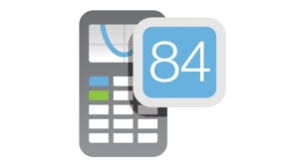
\includegraphics[width=1cm]{TI84Plus-icoon}}}
\newcommand{\grmref}[1]{%
	\reversemarginpar%
	\marginpar{
		\vspace{-0.4cm}%
		\htmladdnormallink{\grmlink}{#1}
	}	
}

% GRM knoppen:
\newcommand{\GRM}[1]{\fbox{\rule[0mm]{0cm}{0.215cm}\textup{\texttt{#1}}}}
\newcommand{\wedgetext}{{\raisebox{0.02cm}{\begin{turn}{90}>\end{turn}}}}
\newcommand{\veetext}{\raisebox{0.2cm}{\begin{turn}{-90}>\end{turn}}}

% voor kolommen met GRM screens:
\newlength{\widthallscreens}
\newlength{\widthscreens}
\newlength{\spaceleftscreen}
\newlength{\spacerightscreen}
\newlength{\spacebetweenscreens}

\newcommand{\setscreens}{
	\setlength{\spaceleftscreen}{2pt}
	\setlength{\spacerightscreen}{2pt}
	\setlength{\spacebetweenscreens}{8pt}
	\addtolength{\linewidth}{-28pt} % 3*8pt tussen vier screens en 2 pt links en 2 pt rechts
	\setlength{\widthallscreens}{\linewidth}
	\setlength{\widthscreens}{0.25\widthallscreens}
	\addtolength{\linewidth}{28pt}
	\newcolumntype{G}{p{\widthscreens}}
	\newcolumntype{s}{p{\spacebetweenscreens}}
	\newcolumntype{L}{p{\spaceleftscreen}}
	\newcolumntype{R}{p{\spacerightscreen}}
	\setlength{\tabcolsep}{0pt}
}

% voor icoon met verwijzing naar Wiskunde Samen gevat² in de marge:
% \newcommand{\wsglink}{\raisebox{0cm}{\includegraphics[width=1cm]{wsglogo}}}
\newcommand{\wsglink}{\raisebox{0cm}{LOGO}}
\newcommand{\htmladdnormallink}[2]{\href{#2}{#1}}
\newcounter{pagnrwsg}
\newcommand{\wsgref}[3]{% 
    % #1 woord dat onderstippeld wordt
    % #2 pagina van Wiskunde Samen gevat² waar je op terecht komt als je op de link klikt  
    % #3 afgedrukt op het logo van Wiskunde Samen gevat² in de marge: één of meerdere paginanummers
    \ifthenelse{\wsg < 1}{#1}{%
        \underdashed{#1}%
        {\setcounter{pagnrwsg}{#2}}%
        {\addtocounter{pagnrwsg}{14}}%
        \reversemarginpar%
        \marginpar{\vspace{-0.6cm}%
           \htmladdnormallink{\wsglink}{https://online.fliphtml5.com/sanky/laea/\#p=\arabic{pagnrwsg}}%
            \raisebox{0.41cm}[0cm][0cm]{%
                \hspace{-1.5cm}\makebox[2cm][c]{\colorbox{white}{\texttt{\footnotesize{#3}}}}%
            }%
        }%
    }%
}

% voor invoegen blanco pagina bij de optie recto-verso:
\def\blancobijrectoverso{
	\ifthenelse{\rectoverso < 1}{\clearpage}{
	\clearpage
	\thispagestyle{empty}
	\mbox{}
	\clearpage
	}
}

% aantal pagina's van het bestand:
\ifthenelse{\rectoverso < 1}{\def\totpag{57}}{\def\totpag{66}}

% documenteigenschappen:
% \usepackage{hyperxmp}
% \hypersetup{
% pdftitle={Open Source Wiskunde Aan zet: Veeltermen}, 
% pdfnumpages={\totpag},
% pdfauthor={Koen De Naeghel},
% pdflang={nl},
% pdfkeywords={wiskunde, open source, wiskunde aan zet, veeltermen, secundair onderwijs, tweede graad, doorstroomfinaliteit},
% pdfsubject={Veeltermen},
% pdfcopyright={\unichar{"24B8} 2024 Koen De Naeghel},
% pdfdate={17 december 2024},
% pdfapart=1,
% pdfstartview=}

% voor het benoemen van titel, auteur en datum:
% \title{Veeltermen}
% \author{Auteur: Koen De Naeghel}
% \date{\today}

\newcommand\BackgroundPic{
    \put(-260,-125){
    \parbox[b][\paperheight]{\paperwidth}{%
    \vfill
    \centering
    
\includegraphics[height=\paperwidth, keepaspectratio]{WaZlogo}%
    \vfill
}}}

% marges:
% \usepackage[paper=a4paper,margin=3.4cm,marginparwidth=2cm]{geometry}
% \usepackage[margin=.5in, includehead, includefoot, hmargin={.8in,.5in}, a4paper]{geometry}
% zes voorkeuren die je meteen zelf kan instellen:
\def\uitbr{1} % waarde 1 als je Uitbreiding in de marge wilt, 0 als je dat niet wilt 
\def\wsg{0} % waarde 1 als je verwijzingen naar Wiskunde Samen gevat² wilt, 0 als je dat niet wilt (onderstippelde woorden in de hoofdtekst en logo met paginanummer en hyperlink naar boekpagina in de marge)
\def\rectoverso{0} % waarde 1 als je het PDF-bestand recto-verso wilt laten afdrukken, 0 als je het recto wilt
\def\voetn{0} % waarde 1 als je de voetnoten wilt, 0 als je dat niet wilt 
\def\grm{0} % waarde 1 als je de schermafdrukken van TI-84 Plus wilt, 0 als je dat niet wilt
\def\grmlogo{0} % waarde 1 als je logo TI-84 Plus in de marge wilt, 0 als je dat niet wilt (met hyperlink naar filmpje) 



% packages algemeen:
\pdfOnly{
% \usepackage[english,dutch]{babel}
}
\usepackage{amsfonts}
\usepackage{amsmath} %  o.a. \eqref en \text, omgeving equation*
\usepackage{amssymb} % o.a. \nmid
\usepackage{amsthm} % o.a. omgeving proof
\usepackage{graphicx} % o.a. figuren
\usepackage{xcolor} % \color
% \usepackage[disable]{todonotes} % \todo 
\usepackage{comment} % omgeving comment
\usepackage{xcolor} % kleuren 
\usepackage[skip=7pt plus1pt, indent=0pt]{parskip} % skip = verticale ruimte tussen twee alinea's, indent = insprong bij nieuwe alinea
\usepackage{multicol} % kolommen
\usepackage{xfrac} % breuken

\usepackage{siunitx} % SI eenheden
\usepackage{eso-pic} % achtergrond voorpagina
\usepackage{tabularx} % kolommen voor rekenmachine
\usepackage{rotating} % voor omgeving turn

% voor figuren met PSTricks:
\usepackage{pstricks} 
\usepackage{pstricks-add}
\usepackage{pst-plot}
\usepackage{pst-node}
\usepackage{pst-coil}
\usepackage{auto-pst-pdf}

% voor figuren met TikZ:
\usepackage{tikz} 
\usepackage{tkz-euclide} 
\usepackage{pgfplots} 
\usetikzlibrary{calc,intersections,through,backgrounds,patterns} 
\pgfplotsset{compat=newest}
\usepgfplotslibrary{fillbetween,colormaps}
\usepackage{import}
\usepackage{tikz-3dplot}

% zelfde parskip in minipage:
\makeatletter
\setlength{\parskip}{\medskipamount}
\newcommand{\@minipagerestore}{\setlength{\parskip}{\medskipamount}}
\makeatother

% voor veranderen van de naam Bibliografie naar Referentielijst:
\pdfOnly{
\addto\captionsdutch{\renewcommand{\bibname}{Referentielijst}}

% voor trefwoordenlijst:
\usepackage{imakeidx}
\makeindex[title=Trefwoordenlijst,program=makeindex,options=-s index.tex,columns=2,intoc=true]
}
% voor nummeren van vergelijkingen:
%WIM%\numberwithin{equation}{chapter} % als je dit desactiveert dan worden vergelijkingen in bijvoorbeeld hoofdstuk 3 genummerd als (1), (2) etc. in plaats van (3.1), (3.2) etc.

% voor hyperlinks en bladwijzers in PDF-bestand:
%WIM%\usepackage[bookmarksopen,bookmarksopenlevel=0,hypertexnames=false,pdfa,bookmarksnumbered]{hyperref} 
%WIM%\usepackage{bookmark} 

% voor hyperlinks: 
\hypersetup{pdfborder={0 0 0}, pdfstartpage=1,linkbordercolor={1 0 0}}%pdfborder={0 0 0} is geen rand rond hyperlinks, pdfborder={1 1 1} wel

% korter commando voor displaystyle, om bijvoorbeeld breuken groter te drukken in doorlopende tekst: 
\newcommand{\D}{\displaystyle}

% (veel)gebruikte verzamelingen:
\newcommand\NN{\mathbb{N}} % verzameling van de natuurlijke getallen
\newcommand\QQ{\mathbb{Q}} % verzameling van de rationale getallen
\newcommand\RR{\mathbb{R}} % verzameling van de re\"ele getallen
\newcommand\ZZ{\mathbb{Z}} % verzameling van de gehele getallen

% (veel)gebruikte operatoren:
\def\co{\operatorname{co}} % coördinaat van een punt
\def\ggd{\operatorname{ggd}} % positieve grootste gemene deler van twee gehele getallen niet beide nul
\def\gr{\operatorname{gr}} % graad van een veelterm

% voor kleur grafieken (donkergroen):
\definecolor{graf}{RGB}{0,100,0} 

% voor lijsten: 
% \usepackage{enumerate}
% \usepackage[shortlabels]{enumitem} 
\setlist{topsep=0em, itemsep=-0.15em}

% voor small bullet:
\newcommand\sbullet[1][.5]{\mathbin{\vcenter{\hbox{\scalebox{#1}{$\bullet$}}}}}

% voor meer verticale ruimte tussen vergelijkingen in align
\addtolength{\jot}{0.1cm}

% voor meervoudige voetnoten:
\usepackage{fnpct}

% voor het onderdrukken van voetnoten als optie:
\usepackage{letltxmacro}
\LetLtxMacro\Oldfootnote\footnote
\newcommand{\EnableFootNotes}{%
  \LetLtxMacro\footnote\Oldfootnote%
}
\newcommand{\DisableFootNotes}{%
  \renewcommand{\footnote}[2][]{\relax}
}

% voor verticale lijn in de marge (uitbreiding):
\usepackage[framemethod=default]{mdframed}
\usepackage{marginnote}
\reversemarginpar
\ifthenelse{\uitbr < 1}{\definecolor{rood}{RGB}{255,255,255}}{\definecolor{rood}{RGB}{254,64,64}} %HEX: #fe4040
\mdfdefinestyle{uitbreiding}{%
    topline=false,
    rightline=false,
    bottomline=false,
    leftline=true,
    linecolor=rood,
    linewidth=5pt,
    rightmargin=0pt,
    skipabove=10pt,% ipv 3
    skipbelow=0pt,
    leftmargin=-25pt,
    innerleftmargin=20pt,
    innerrightmargin=0pt,
    innertopmargin=0pt,
    innerbottommargin=0pt%,
%	needspace=30pt %minimumhoogte vooraleer lijn wordt gesplitst
    }
% \newenvironment{Uitbreiding}{
%     \marginpar{
%         \center
% 		\vspace{0.1cm}
% 		\vspace{7pt}
% 		\rotatebox{90}{\color{rood}\Large \bf Uitbreiding}
% 	}
%     \begin{mdframed}[style=uitbreiding]
%     }{\vspace{-0.05cm}
%     \end{mdframed}
% }

\newenvironment{Uitbreiding}{\begin{xmuitweiding}}{\end{xmuitweiding}}
% omgevingen voor lemma, definitie, voorbeeld etc.:
\newtheoremstyle{mystyle}
    {0em} % Space above
    {0em} % Space below
    {\itshape} % Body font
    {} % Indent amount
    {\bfseries} % Theorem head font
    {.} % Punctuation after theorem head
    {.5em} % Space after theorem head
    {} % Theorem head spec (can be left empty, meaning `normal')
\theoremstyle{mystyle}
%WIM%\newtheorem{lemma}{Lemma}[chapter] % als je [chapter] desactiveert dan Voorbeeld 3 in plaats van Voorbeeld 5.3, als je [chapter] vervangt door [section] dan Voorbeeld 5.2.3 in plaats van Voorbeeld 5.3 
%\theoremstyle{definition} % als je dit activeert dan is wat in de omgeving staat niet cursief gedrukt
\newtheorem{oefening}[lemma]{Oefening}
\newtheorem{definitie}[lemma]{Definitie} 
\newtheorem{voorbeeld}[lemma]{Voorbeeld}
\newtheorem{eigenschap}[lemma]{Eigenschap} 
\newtheorem{stelling}[lemma]{Stelling} 
\newtheorem{gevolg}[lemma]{Gevolg} 
\newtheorem{afspraak}[lemma]{Afspraak} 
\newtheorem{werkwijze}[lemma]{Werkwijze}

% omgeving proof, aangepaste ruimte: 
\makeatletter
\renewenvironment{proof}[1][\proofname]{\par
  \vspace{-\topsep}% remove the space after the theorem
  \pushQED{\qed}%
  \normalfont
  \topsep0pt \partopsep0pt % no space before
  \trivlist
  \item[\hskip\labelsep
        \itshape
    #1\@addpunct{.}]\ignorespaces
}{%
  \popQED\endtrivlist\@endpefalse
  \addvspace{0pt plus 0pt} % no space after
}
\makeatother

% kaderstijlen uit SOHO Wiskunde Plantyn:
\colorlet{steunkleur}{black}
\colorlet{steunkleurlicht}{steunkleur!30!white}
\colorlet{steunkleurkader}{steunkleur!7!white}
\colorlet{steunkleurkaderlicht}{steunkleur!2!white}

\mdfdefinestyle{kaderstijl_vol_licht}
{skipabove=6pt, 
skipbelow=6pt, 
backgroundcolor=steunkleurkader,
linecolor=steunkleurlicht,
linewidth = 0.4pt, 
topline=true,
bottomline=true, 
rightline=true,
innerleftmargin=5pt,
innerrightmargin=5pt,
innertopmargin=5pt,
leftmargin=0cm,
rightmargin=0cm,
innerbottommargin=5pt,
needspace=30pt % minimumhoogte voor splitsen kader
}
\surroundwithmdframed[style=kaderstijl_vol_licht]{definitie}
\surroundwithmdframed[style=kaderstijl_vol_licht]{stelling}
\surroundwithmdframed[style=kaderstijl_vol_licht]{lemma}
\surroundwithmdframed[style=kaderstijl_vol_licht]{eigenschap}
\surroundwithmdframed[style=kaderstijl_vol_licht]{gevolg}

% voor omgevingen voor oefening en antwoord:
\newenvironment{Oefening}{%
    \begin{enumerate}[ 
    series=Oef,
    resume=Oef,
    leftmargin=1.78em,
    label={\bfseries\arabic*.},
    ref=\arabic*
    ]
    \item %
    }{%
    \end{enumerate}
}
\newenvironment{Antwoord}{%
    \begin{enumerate}[%
    series=Antw,
    resume=Antw,
    leftmargin=1.78em,
    label={\bfseries\arabic*.},
    ref=\arabic*
    ]
    \item %
    }{%
    \end{enumerate}
}

% als de omgeving Uitbreiding start met een kaderomgeving (definitie, stelling, eigenschap, lemma of gevolg) dan moet wat extra verticale ruimte voorzien worden, met het commando \uitbreidingstartmetkader:
\def\uitbreidingstartmetkader{\mbox{}\vspace{-0.205cm}}

%WIM % voor schema van de staartdeling:
\usepackage{stackengine}
\setstackgap{S}{5pt}
\stackMath\def\stackalignment{r}
\newcommand{\myRule}[3][white]{\textcolor{#1}{\rule{#2}{#3}}}
\let\ph\phantom % enkel voor tekst
\newcommand{\mph}[1]{% enkel voor math mode
    \mathcolor{white}{#1}%
}
\def\staartmin{\rule{0.25cm}{0.1mm}\myRule{0.3cm}{0.1mm}}
\def\staartphmin{\myRule{0.25cm}{0.1mm}\myRule{0.3cm}{0.1mm}}
\newcommand{\staartstreep}[1]{\rule{\widthof{$#1$}}{0.1mm}}
\newcommand{\staartphstreep}[1]{\myRule{\widthof{$#1$}}{0.1mm}}

% voor kolommen met schema van Horner:
\newcommand{\kolbreed}{1.0cm}
\newcolumntype{H}{>{\centering\arraybackslash$} p{\kolbreed} <{$}}

% voor nieuw commando utikzdashed: onderlijn (zoals underline) maar dan met stippellijn:
\tikzset{
    cheating dash/.code args={on #1 off #2 ends #3}{%
        \csname tikz@addoption\endcsname{%
            \pgfgetpath\currentpath%
            \pgfprocessround{\currentpath}{\currentpath}%
            \csname pgf@decorate@parsesoftpath\endcsname{\currentpath}{\currentpath}%
            \pgfmathparse{max(#1-#3,0)}\let\dashphase=\pgfmathresult%
            \pgfmathparse{\csname pgf@decorate@totalpathlength\endcsname-#1+2*\dashphase}\let\rest=\pgfmathresult%
            \pgfmathparse{#1+#2}\let\onoff=\pgfmathresult%
            \pgfmathparse{max(floor(\rest/\onoff), 1)}\let\nfullonoff=\pgfmathresult%
            \pgfmathparse{max((\rest-\onoff*\nfullonoff)/\nfullonoff+#2, #2)}\let\offexpand=\pgfmathresult%
            \pgfsetdash{{#1}{\offexpand}}{\dashphase pt}}%
    },
    cheating dash per segment/.style args={on #1 off #2 ends #3}{
        /utils/exec=\csname tikz@options\endcsname,%
        decoration={show path construction,
            lineto code={\draw [cheating dash=on #1 off #2 ends #3] (\tikzinputsegmentfirst) -- (\tikzinputsegmentlast);},
            curveto code={\draw [cheating dash=on #1 off #2 ends #3] (\tikzinputsegmentfirst) .. controls (\tikzinputsegmentsupporta) and (\tikzinputsegmentsupportb) .. (\tikzinputsegmentlast);},
            closepath code={\draw [cheating dash=on #1 off #2 ends #3] (\tikzinputsegmentfirst) -- (\tikzinputsegmentlast);}
        },
        decorate,
    },
}
\newcommand{\utikzdash}[1]{%
    \tikz[baseline=(todotted.base)]{
        \node[inner sep=0pt,outer sep=1.5pt] (todotted) {#1};
        \draw[cheating dash per segment=on 2pt off 2pt ends 2pt, line width=0.4pt] (todotted.south west) -- (todotted.south east);
    }%
}%

% voor nieuw commando underdashed: onderlijn met stippellijnen en ook het woord cursief zetten:
\newcommand{\underdashed}[1]{%
    {\em\utikzdash{\!#1\!}}%
}

% voor icoon TI-84 Plus met verwijzing naar filmpje:
\newcommand{\grmlink}{\raisebox{0cm}{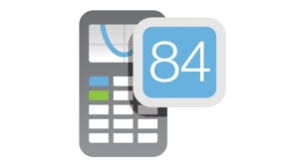
\includegraphics[width=1cm]{TI84Plus-icoon}}}
\newcommand{\grmref}[1]{%
	\ifthenelse{\grmlogo < 1}{}{
		\reversemarginpar%
		\marginpar{
			\vspace{-0.4cm}%
			\htmladdnormallink{\grmlink}{#1}
		}
	}	
}

% GRM knoppen:
\newcommand{\GRM}[1]{\fbox{\rule[0mm]{0cm}{0.215cm}\textup{\texttt{#1}}}}
\newcommand{\wedgetext}{{\raisebox{0.02cm}{\begin{turn}{90}>\end{turn}}}}
\newcommand{\veetext}{\raisebox{0.2cm}{\begin{turn}{-90}>\end{turn}}}

% voor kolommen met GRM screens:
\newlength{\widthallscreens}
\newlength{\widthscreens}
\newlength{\spaceleftscreen}
\newlength{\spacerightscreen}
\newlength{\spacebetweenscreens}

\newcommand{\setscreens}{
	\setlength{\spaceleftscreen}{2pt}
	\setlength{\spacerightscreen}{2pt}
	\setlength{\spacebetweenscreens}{8pt}
	\addtolength{\linewidth}{-28pt} % 3*8pt tussen vier screens en 2 pt links en 2 pt rechts
	\setlength{\widthallscreens}{\linewidth}
	\setlength{\widthscreens}{0.25\widthallscreens}
	\addtolength{\linewidth}{28pt}
	\newcolumntype{G}{p{\widthscreens}}
	\newcolumntype{s}{p{\spacebetweenscreens}}
	\newcolumntype{L}{p{\spaceleftscreen}}
	\newcolumntype{R}{p{\spacerightscreen}}
	\setlength{\tabcolsep}{0pt}
}

% voor icoon met verwijzing naar Wiskunde Samen gevat² in de marge:
\newcommand{\wsglink}{\raisebox{0cm}{\includegraphics[width=1cm]{wsglogo}}}
\newcommand{\htmladdnormallink}[2]{\href{#2}{#1}}
\newcounter{pagnrwsg}
\newcommand{\wsgref}[3]{% 
    % #1 woord dat onderstippeld wordt
    % #2 pagina van Wiskunde Samen gevat² waar je op terecht komt als je op de link klikt  
    % #3 afgedrukt op het logo van Wiskunde Samen gevat² in de marge: één of meerdere paginanummers
    \ifthenelse{\wsg < 1}{#1}{%
        \underdashed{#1}%
        {\setcounter{pagnrwsg}{#2}}%
        {\addtocounter{pagnrwsg}{14}}%
        \reversemarginpar%
        \marginpar{\vspace{-0.6cm}%
           \htmladdnormallink{\wsglink}{https://online.fliphtml5.com/sanky/laea/\#p=\arabic{pagnrwsg}}%
            \raisebox{0.41cm}[0cm][0cm]{%
                \hspace{-1.5cm}\makebox[2cm][c]{\colorbox{white}{\texttt{\footnotesize{#3}}}}%
            }%
        }%
    }%
}

% voor invoegen blanco pagina bij de optie recto-verso:
\def\blancobijrectoverso{
	\ifthenelse{\rectoverso < 1}{\clearpage}{
	\clearpage
	\thispagestyle{empty}
	\mbox{}
	\clearpage
	}
}

% aantal pagina's van het bestand:
\ifthenelse{\rectoverso < 1}{\def\totpag{57}}{\def\totpag{66}}

% documenteigenschappen:
% \usepackage{hyperxmp}
% \hypersetup{
% pdftitle={Open Source Wiskunde Aan zet: Veeltermen}, 
% pdfnumpages={\totpag},
% pdfauthor={Koen De Naeghel},
% pdflang={nl},
% pdfkeywords={wiskunde, open source, wiskunde aan zet, veeltermen, secundair onderwijs, tweede graad, doorstroomfinaliteit},
% pdfsubject={Veeltermen},
% pdfcopyright={\unichar{"24B8} 2024 Koen De Naeghel},
% pdfdate={17 december 2024},
% pdfapart=1,
% pdfstartview=}

% voor het benoemen van titel, auteur en datum:
% \title{Veeltermen}
% \author{Auteur: Koen De Naeghel}
% \date{\today}

\newcommand\BackgroundPic{
    \put(-260,-125){
    \parbox[b][\paperheight]{\paperwidth}{%
    \vfill
    \centering
    
\includegraphics[height=\paperwidth, keepaspectratio]{WaZlogo}%
    \vfill
}}}


\newcommand{\chapter}{\section}

\addPrintStyle{.}

\begin{document}
	\author{Koen De Naeghel}
	\xmtitle{Eindantwoorden}{}
	\label{xim:veeltermen_eindantwoorden}
\chapter{Eindantwoorden van oefeningen}
\section*{Hoofdstuk 1}

\begin{Antwoord} \label{antw1.1}
\begin{enumerate}

\item
\hyperlink{oef1.1}{eenterm}
\item
\hyperlink{oef1.1}{eenterm}
\item
\hyperlink{oef1.1}{geen eenterm}
\item
\hyperlink{oef1.1}{eenterm}
\item
\hyperlink{oef1.1}{geen eenterm}
\item
\hyperlink{oef1.1}{eenterm}
\item\hyperlink{oef1.1}{eenterm}
\item
\hyperlink{oef1.1}{eenterm}
\item
\hyperlink{oef1.1}{geen eenterm}
\item
\hyperlink{oef1.1}{geen eenterm}
\end{enumerate}
\end{Antwoord}

\begin{Antwoord} \label{antw1.2}
\begin{enumerate}
\item
\hyperlink{oef1.2}{$x + 2x^2 + 3x^3$}
\item
\hyperlink{oef1.2}{$x + \frac{1}{2}\,x^3 + \frac{1}{3}\,x^5 + \frac{1}{4}\,x^7$}
\item
\hyperlink{oef1.2}{$x^2 - x^3 + x^4$}
\end{enumerate}
\end{Antwoord}

\begin{Antwoord} \label{antw1.3}
\begin{enumerate}
\item
\hyperlink{oef1.3}{veelterm}
\item
\hyperlink{oef1.3}{veelterm}
\item
\hyperlink{oef1.3}{veelterm}
\item
\hyperlink{oef1.3}{veelterm}
\item
\hyperlink{oef1.3}{veelterm}
\item
\hyperlink{oef1.3}{veelterm}
\item
\hyperlink{oef1.3}{geen veelterm}
\item
\hyperlink{oef1.3}{veelterm}
\item
\hyperlink{oef1.3}{veelterm}
\item
\hyperlink{oef1.3}{geen veelterm}
\item
\hyperlink{oef1.3}{veelterm}
\item
\hyperlink{oef1.3}{veelterm}
\end{enumerate}
\setcounter{enumi}{4}
\end{Antwoord}

%%% \clearpage

\begin{Antwoord} \label{antw1.5}
\begin{enumerate}
\item
\hyperlink{oef1.5}{graad $5$, hoogstegraadsco\"effici\"ent $1$, constante term $-15$}
\item
\hyperlink{oef1.5}{graad $6$, hoogstegraadsco\"effici\"ent $2$, constante term $3$}
\item
\hyperlink{oef1.5}{graad $7$, hoogstegraadsco\"effici\"ent $\frac{2}{3}$, constante term $-\frac{3}{7}$}
\item
\hyperlink{oef1.5}{graad $6$, hoogstegraadsco\"effici\"ent $-15$, constante term $-70$}
\item
\hyperlink{oef1.5}{graad $3$, hoogstegraadsco\"effici\"ent $125$, constante term $0$}
\item
\hyperlink{oef1.5}{graad $6$, hoogstegraadsco\"effici\"ent $64$, constante term $125$}
\end{enumerate}
\setcounter{enumi}{6}
\end{Antwoord}

\begin{Antwoord} \label{antw1.7}
\begin{enumerate}
\item
\hyperlink{oef1.7}{$-x^3+x^2+3x+1$, graad $3$}
\item
\hyperlink{oef1.7}{$x^3-5x^2+4x$, graad $3$}
\item
\hyperlink{oef1.7}{$\sqrt{10}\,x+\sqrt{15}$, graad $1$}
\item
\hyperlink{oef1.7}{$-9x^4+45x^3+3x^2-21x+30$, graad $4$}
\item
\hyperlink{oef1.7}{$-\frac{4}{5}\,x^2-\frac{1}{5}\,x-\frac{4}{5}$, graad $2$}
\item
\hyperlink{oef1.7}{$4x-8$, graad $1$}
\item
\hyperlink{oef1.7}{$-8x^2+18$, graad $2$}
\item
\hyperlink{oef1.7}{$\frac{15}{2}\,x^3 + 3x^2 - \frac{10}{3}\,x-\frac{4}{3}$, graad $3$}
\end{enumerate}
\end{Antwoord}

\begin{Antwoord} \label{antw1.8}
\begin{enumerate}
\item
\hyperlink{oef1.8}{$A(2)=0$, nulwaarde}
\item
\hyperlink{oef1.8}{$B(-1)=1$, geen nulwaarde}
\item
\hyperlink{oef1.8}{$P(5)=0$, nulwaarde}
\item
\hyperlink{oef1.8}{$S(0)=-1$, geen nulwaarde}
\item
\hyperlink{oef1.8}{$C(\sqrt{2})=0$, nulwaarde}
\item
\hyperlink{oef1.8}{$D\left(-\frac{1}{2}\right)=0$, nulwaarde}
\end{enumerate}
\end{Antwoord}

\begin{Antwoord} \label{antw1.9}
\begin{enumerate}
\item
\hyperlink{oef1.9}{$a=-3$}
\item
\hyperlink{oef1.9}{$a = 1$ en $b = -3$}
\end{enumerate}
\end{Antwoord}

\begin{Antwoord} \label{antw1.10}
\begin{enumerate}
\item
\hyperlink{oef1.10}{$a = -\frac{3}{2}$}
\item
\hyperlink{oef1.10}{$c = \frac{2}{1-\sqrt{2}}$}
\end{enumerate}
\end{Antwoord}

\begin{Antwoord} \label{antw1.11}
\begin{enumerate}
\item
\hyperlink{oef1.11}{$A(x) = -3x^6+24x^4+12x^2$ en $B(x) = -5x^2$}
\item
\hyperlink{oef1.11}{$\gr A(x) = 6$ en $\gr B(x) = 2$}
\item
\hyperlink{oef1.11}{$A(-2) = 240$ en $B(\sqrt{3}) = -15$}
\end{enumerate}
\end{Antwoord}


\begin{Antwoord} \label{antw1.12}
\begin{enumerate}
\item
\hyperlink{oef1.12}{$475$}
\item
\hyperlink{oef1.12}{$c = -2$}
\end{enumerate}
\end{Antwoord}

\begin{Antwoord} \label{antw1.13}
\hyperlink{oef1.13}{$A(x) = -x^2-x+2$}
\end{Antwoord}

\begin{Antwoord} \label{antw1.14}
\hyperlink{oef1.14}{$A(x) = \frac{1}{3}\,x^3-\frac{1}{3}\,x$}
\end{Antwoord}

\begin{Antwoord} \label{antw1.15}
\hyperlink{oef1.15}{$2x^2+3x+1$}
\end{Antwoord}

\begin{Antwoord} \label{antw1.16}
\hyperlink{oef1.16}{$a = 3$ en $b = \frac{1}{4}$}
\end{Antwoord}

\begin{Antwoord} \label{antw1.17}
\hyperlink{oef1.17}{$4096$}
\end{Antwoord}

\begin{Antwoord} \label{antw1.18}
\hyperlink{oef1.18}{$32$}
\setcounter{enumi}{0}
\end{Antwoord}

%%% \clearpage

\section*{Hoofdstuk 2}

\begin{Antwoord} \label{antw2.1}
\begin{enumerate}

\item
\hyperlink{oef2.1}{deelbaar, quoti\"ent $6x^2$} 
\item
\hyperlink{oef2.1}{deelbaar, quoti\"ent $-2$}
\item
\hyperlink{oef2.1}{deelbaar, quoti\"ent $\frac{3}{2}\,x^4$}
\item
\hyperlink{oef2.1}{deelbaar, quoti\"ent $0$}
\item
\hyperlink{oef2.1}{niet deelbaar}
\item
\hyperlink{oef2.1}{deelbaar, quoti\"ent $-\frac{1}{10}\,x$}
\item
\hyperlink{oef2.1}{deelbaar, quoti\"ent $\frac{\sqrt{2}}{6}$}
\item
\hyperlink{oef2.1}{niet deelbaar}
\end{enumerate}
\end{Antwoord}

\begin{Antwoord} \label{antw2.2}
\begin{enumerate}
\item
\hyperlink{oef2.2}{deelbaar door $6$, quoti\"ent $2x^3 - 3x^2 + x$} 
\item[]
\hyperlink{oef2.2}{deelbaar door $3x$, quoti\"ent $4x^2 - 6x + 2$} 
\item[]
\hyperlink{oef2.2}{niet deelbaar door $3x^2$}
\item
\hyperlink{oef2.2}{deelbaar door $6$, quoti\"ent $x^2 - \frac{1}{2}\,x$} 
\item[]
\hyperlink{oef2.2}{deelbaar door $3x$, quoti\"ent $2x-1$} 
\item[]
\hyperlink{oef2.2}{niet deelbaar door $3x^2$}
\item
\hyperlink{oef2.2}{deelbaar door $6$, quoti\"ent $0$} 
\item[]
\hyperlink{oef2.2}{deelbaar door $3x$, quoti\"ent $0$} 
\item[]
\hyperlink{oef2.2}{niet deelbaar door $0$}
\item
\hyperlink{oef2.2}{deelbaar door $6$, quoti\"ent $\frac{1}{3}\,x^3 + \frac{1}{10}\,x^2$} 
\item[]
\hyperlink{oef2.2}{deelbaar door $3x$, quoti\"ent $\frac{2}{3}\,x^2 + \frac{1}{5}\,x$} 
\item[]
\hyperlink{oef2.2}{deelbaar door $3x^2$, quoti\"ent $\frac{2}{3}\,x + \frac{1}{5}$}
\item
\hyperlink{oef2.2}{deelbaar door $6$, quoti\"ent $\frac{\sqrt{3}}{6}\,x - \frac{4}{3}$} 
\item[]
\hyperlink{oef2.2}{niet deelbaar door $3x$}
\item[]
\hyperlink{oef2.2}{niet deelbaar door $3x^2$}
\item
\hyperlink{oef2.2}{deelbaar door $6$, quoti\"ent $\frac{1}{6}\,x^8 - \frac{\pi}{6}\,x^5$} 
\item[]
\hyperlink{oef2.2}{deelbaar door $3x$, quoti\"ent $\frac{1}{3}\,x^7 - \frac{\pi}{3}\,x^4$} 
\item[]
\hyperlink{oef2.2}{deelbaar door $3x^2$, quoti\"ent $\frac{1}{3}\,x^6 - \frac{\pi}{3}\,x^3$}
\end{enumerate}
\end{Antwoord}

\begin{Antwoord} \label{antw2.3}
\hyperlink{oef2.3}{$-3x^3+11x^2-5x+2$}
\end{Antwoord}

\begin{Antwoord} \label{antw2.4}
\hyperlink{oef2.4}{$p=2$ en $q=8$}
\end{Antwoord}

\begin{Antwoord} \label{antw2.5}
\begin{enumerate}
\item
\hyperlink{oef2.5}{quoti\"ent $5$, rest $3x$, niet deelbaar, verband $A(x) = 5B(x)+3x$}
\item
\hyperlink{oef2.5}{quoti\"ent $x$, rest $0$, deelbaar, verband $A(x) = xB(x)+0$}
\item
\hyperlink{oef2.5}{quoti\"ent $\frac{5}{2}\,x$, rest $2$, niet deelbaar, verband $A(x) = \frac{5}{2}\,xB(x)+2$}
\item
\hyperlink{oef2.5}{quoti\"ent $-\frac{3}{5}$, rest $0$, deelbaar, verband $A(x) = -\frac{3}{5}\,B(x)+0$}
\item
\hyperlink{oef2.5}{quoti\"ent $0$, rest $7x^2-8x+5$, niet deelbaar, verband $A(x) = 0B(x)+7x^2-8x+5$}
\item
\hyperlink{oef2.5}{quoti\"ent $3$, rest $10x-72$, niet deelbaar, verband $A(x) = 3B(x)+10x-72$}
\item
\hyperlink{oef2.5}{quoti\"ent $-\frac{8}{3}\,x$, rest $16$, niet deelbaar, verband $A(x) = -\frac{8}{3}\,xB(x)+16$}
\end{enumerate}
\end{Antwoord}

\begin{Antwoord} \label{antw2.6}
\hyperlink{oef2.6}{$12$}
\end{Antwoord}

\begin{Antwoord} \label{antw2.7}
\begin{enumerate}
\item
\hyperlink{oef2.7}{niet deelbaar}
\item
\hyperlink{oef2.7}{niet deelbaar}
\item
\hyperlink{oef2.7}{deelbaar}
\item
\hyperlink{oef2.7}{deelbaar}
\item
\hyperlink{oef2.7}{niet deelbaar}
\end{enumerate}
\end{Antwoord}

\begin{Antwoord} \label{antw2.8}
\begin{enumerate}
\item
\hyperlink{oef2.8}{$x^4 + x^2 + 1 = (x^2+x+1)(x^2-x+1)$}
\item
\hyperlink{oef2.8}{$x^5 - 1 = (x-1)(x^4+x^3+x^2+x+1)$}
\item
\hyperlink{oef2.8}{$x^4 + 1 = (x^2+\sqrt{2}\,x+1)(x^2-\sqrt{2}\,x+1)$}
\end{enumerate}
\end{Antwoord}

\begin{Antwoord} \label{antw2.9}
\begin{enumerate}
\item
\hyperlink{oef2.9}{$a=2$ en $b = 2$}
\item
\hyperlink{oef2.9}{$a = 22$ en $b = -8$}
\item
\hyperlink{oef2.9}{$a = 0$ en $b = 2$}
\item
\hyperlink{oef2.9}{$a = 4$, $b = 3$ en $c = 5$}
\item
\hyperlink{oef2.9}{$a \in \left\{\sqrt{2},-\sqrt{2}\right\}$ en $b = 1$}
\item
\hyperlink{oef2.9}{$a \in \left\{1,-1\right\}$ en $b = 1$}
\end{enumerate}
\end{Antwoord}

\begin{Antwoord} \label{antw2.10}
\begin{enumerate}
\item
\hyperlink{oef2.10}{quoti\"ent $x-1$, rest $0$, deelbaar, verband $A(x) = (x-1)B(x)+0$}
\item
\hyperlink{oef2.10}{quoti\"ent $-\frac{1}{3}\,x - \frac{4}{3}$, rest $0$, deelbaar, verband $A(x) = \left(-\frac{1}{3}\,x - \frac{4}{3}\right)B(x)+0$}
\item
\hyperlink{oef2.10}{quoti\"ent $x+5$, rest $0$, deelbaar, verband $A(x) = (x+5)B(x)+0$}
\item
\hyperlink{oef2.10}{quoti\"ent $3x+2$, rest $2x+7$, niet deelbaar, verband $A(x) = (3x+2)B(x)+2x+7$}
\item
\hyperlink{oef2.10}{quoti\"ent $x-1$, rest $7x+3$, niet deelbaar, verband $A(x) = (x-1)B(x)+7x+3$}
\item
\hyperlink{oef2.10}{quoti\"ent $\frac{1}{3}\,x + \frac{5}{9}$, rest $\frac{19}{9}$, niet deelbaar, verband $A(x) = \left(\frac{1}{3}\,x + \frac{5}{9}\right)B(x)+\frac{19}{9}$}
\item
\hyperlink{oef2.10}{quoti\"ent $\frac{1}{2}\,x + \frac{1}{4}$, rest $-\frac{5}{2}\,x - \frac{1}{4}$, niet deelbaar, verband $A(x) = \left( \frac{1}{2}\,x + \frac{1}{4} \right)B(x)-\frac{5}{2}\,x - \frac{1}{4}$}
\end{enumerate}
\end{Antwoord}

\begin{Antwoord} \label{antw2.11}
\begin{enumerate}
\item
\hyperlink{oef2.11}{quoti\"ent $\frac{1}{2}\,x^2 - \frac{1}{2}\,x + \frac{1}{2}$, rest $0$, deelbaar, verband $A(x) = \left(\frac{1}{2}\,x^2 - \frac{1}{2}\,x + \frac{1}{2}\right)B(x)+0$}
\item
\hyperlink{oef2.11}{quoti\"ent $10x^2-3x+23$, rest $-46$, niet deelbaar,} 
\item[]
\hyperlink{oef2.11}{verband $A(x) = \left(10x^2-3x+23\right)B(x)-46$}
\item
\hyperlink{oef2.11}{quoti\"ent $x^2-20$, rest $99x^2+117x-15$, niet deelbaar,} 
\item[]
\hyperlink{oef2.11}{verband $A(x) = (x^2-20)B(x)+99x^2+117x-15$}
\item
\hyperlink{oef2.11}{quoti\"ent $3x^3 + 2x^2 + x + 2$, rest $0$, deelbaar, verband $A(x) = (3x^3 + 2x^2 + x + 2)B(x)+0$} 
\item
\hyperlink{oef2.11}{quoti\"ent $x^3+2x^2+3x+4$, rest $1914$, niet deelbaar,}
\item[]
\hyperlink{oef2.11}{verband $A(x) = (x^3+2x^2+3x+4)B(x)+1914$}
\item
\hyperlink{oef2.11}{quoti\"ent $\frac{1}{3}\,x^2 + \frac{8}{9}$, rest $0$, deelbaar, verband $A(x) = \left(\frac{1}{3}\,x^2 + \frac{8}{9}\right)B(x)+0$}
\item
\hyperlink{oef2.11}{quoti\"ent $x^2 + \frac{1}{2}\,x + \frac{17}{4}$, rest $-\frac{33}{4}\,x + \frac{113}{4}$, niet deelbaar,}
\item[]
\hyperlink{oef2.11}{verband $A(x) = \left( x^2 + \frac{1}{2}\,x + \frac{17}{4} \right)B(x)-\frac{33}{4}\,x + \frac{113}{4}$}
\end{enumerate}
\end{Antwoord}

\begin{Antwoord} \label{antw2.12}
\begin{enumerate}
\item
\hyperlink{oef2.12}{quoti\"ent $4x^2+10$ en rest $ax+b-20$} 
\item
\hyperlink{oef2.12}{quoti\"ent $4x^2-6x+\frac{1}{2}\,a+9$ en rest $-\frac{3}{2}\,a+b-27$} 
\end{enumerate}
\end{Antwoord}

\begin{Antwoord} \label{antw2.13}
\hyperlink{oef2.13}{$m = 0$ en $n = -1$}
\setcounter{enumi}{16}
\end{Antwoord}

\begin{Antwoord} \label{antw2.17}
\hyperlink{oef2.17}{$\gr Q(x) \in \left\{0,1,2,3,4,5,6,7,8,9\right\}$}
\end{Antwoord}

\begin{Antwoord} \label{antw2.18}
\hyperlink{oef2.18}{$a=-2$}
\end{Antwoord}

\begin{Antwoord} \label{antw2.19}
\hyperlink{oef2.19}{$x$}
\end{Antwoord}

\begin{Antwoord} \label{antw2.20}
\begin{enumerate}
\item
\hyperlink{oef2.20}{$Q(x) = 0$ en $R(x) = 0$}
\item
\hyperlink{oef2.20}{$Q(x) = A(x)$ en $R(x) = 0$}
\item
\hyperlink{oef2.20}{$Q(x) = -\frac{1}{7}$ en $R(x) = 0$}
\item
\hyperlink{oef2.20}{$Q(x) = 0$ en $R(x) = A(x)$}
\item
\hyperlink{oef2.20}{$Q(x) = 1$ en $R(x) = 0$}
\item
\hyperlink{oef2.20}{$Q(x) = \frac{1}{\sqrt{2}}$ en $R(x) =-\frac{\pi}{\sqrt{2}}$}
\end{enumerate}
\setcounter{enumi}{0}
\end{Antwoord}

\section*{Hoofdstuk 3}

\begin{Antwoord} \label{antw3.1}
\begin{enumerate}

\item
\hyperlink{oef3.1}{$30$}
\item
\hyperlink{oef3.1}{$0$}
\item
\hyperlink{oef3.1}{$6-14\sqrt{2}$}
\item
\hyperlink{oef3.1}{$6$}
\item
\hyperlink{oef3.1}{$\frac{242}{27}$}
\item
\hyperlink{oef3.1}{$0$}
\end{enumerate}
\end{Antwoord}

\begin{Antwoord} \label{antw3.2}
\hyperlink{oef3.2}{(A)}
\end{Antwoord}

\begin{Antwoord} \label{antw3.3}
\begin{enumerate}
\item
\hyperlink{oef3.3}{geen deler}
\item
\hyperlink{oef3.3}{deler}
\item
\hyperlink{oef3.3}{deler}
\item
\hyperlink{oef3.3}{geen deler}
\end{enumerate}
\end{Antwoord}

\begin{Antwoord} \label{antw3.4}
\begin{enumerate}
\item
\hyperlink{oef3.4}{quoti\"ent $2x^2+11x+33$ en rest $96$}
\item
\hyperlink{oef3.4}{quoti\"ent $x^4-2x^3+3x^2-4x+5$ en rest $-6$}
\end{enumerate}
\end{Antwoord}

\begin{Antwoord} \label{antw3.5}
\hyperlink{oef3.5}{$k = - \frac{153}{40}$}
\end{Antwoord}

\begin{Antwoord} \label{antw3.6}
\hyperlink{oef3.6}{(B)}
\end{Antwoord}

\begin{Antwoord} \label{antw3.7}
\begin{enumerate}
\item
\hyperlink{oef3.7}{$a \in \left\{\frac{1}{2}, -\frac{7}{10}\right\}$}
\item
\hyperlink{oef3.7}{geen enkel re\"eel getal $a$ voldoet}
\item
\hyperlink{oef3.7}{$a = \frac{5+2\sqrt{2}}{3}$}
\item
\hyperlink{oef3.7}{$a \in \RR$}
\item
\hyperlink{oef3.7}{$a = 10$ en $b = -82$}
\item
\hyperlink{oef3.7}{$a = -2$ en $b = 0$}
\item
\hyperlink{oef3.7}{$a = 0$ of $b = 3$}
\end{enumerate}
\end{Antwoord}

\begin{Antwoord} \label{antw3.8}
\hyperlink{oef3.8}{(B)}
\end{Antwoord}

\begin{Antwoord} \label{antw3.9}
\hyperlink{oef3.9}{(C)}
\end{Antwoord}

\begin{Antwoord} \label{antw3.10}
\hyperlink{oef3.10}{$a = 8$ en $b = 19$}
\end{Antwoord}

\begin{Antwoord} \label{antw3.11}
\hyperlink{oef3.11}{(D)}
\end{Antwoord}

\begin{Antwoord} \label{antw3.12}
\hyperlink{oef3.12}{$A(x) = (b-c)(x-b)(x-c)$}
\end{Antwoord}

\begin{Antwoord} \label{antw3.13}
\hyperlink{oef3.13}{(C)}
\end{Antwoord}

\begin{Antwoord} \label{antw3.14}
\begin{enumerate}
\item
\hyperlink{oef3.14}{quoti\"ent $2x^2+6x+15$ en rest $92$}
\item
\hyperlink{oef3.14}{quoti\"ent $18x^2 - 18\sqrt{6}\,x+108$ en rest $-10-108\sqrt{6}$}
\item
\hyperlink{oef3.14}{quoti\"ent $2x^3+16x^2-8x-64$ en rest $32$}
\item
\hyperlink{oef3.14}{quoti\"ent $\sqrt{2}\,x+4\sqrt{10}$ en rest $0$}
\end{enumerate}
\end{Antwoord}

\begin{Antwoord} \label{antw3.15}
\begin{enumerate}
\item[(b)]
\hyperlink{oef3.15}{quoti\"ent $3x^3-2x^2+10x-7$ en rest $-20$}
\end{enumerate}
\end{Antwoord}

\begin{Antwoord} \label{antw3.16}
\hyperlink{oef3.16}{$12x-6$}
\setcounter{enumi}{19}
\end{Antwoord}

\begin{Antwoord} \label{antw3.20}
\hyperlink{oef3.20}{$100$}
\setcounter{enumi}{0}
\end{Antwoord}

\section*{Hoofdstuk 4}

\begin{Antwoord} \label{antw4.1}
\begin{enumerate}

\item
\hyperlink{oef4.1}{$21x^{10}$}
\item
\hyperlink{oef4.1}{$-\frac{9}{50}\,x^7$}
\item
\hyperlink{oef4.1}{$-\frac{1}{2}\,x^6 + 3x^5 + 4x^4 - x^3 + \frac{1}{2}\,x^2$}
\item
\hyperlink{oef4.1}{$x^5 - 5x^4 + 10x^3 - 10x^2 + 5x - 1$}
\end{enumerate}
\end{Antwoord}

\begin{Antwoord} \label{antw4.2}
\begin{enumerate}
\item
\hyperlink{oef4.2}{$3x^2 - 4$}
\item
\hyperlink{oef4.2}{$x^4-1$}
\item
\hyperlink{oef4.2}{$x^6-9$}
\item
\hyperlink{oef4.2}{$4x^6 + \frac{4}{3}\,x^3+\frac{1}{9}$}
\item
\hyperlink{oef4.2}{$1 + 2x + x^2 - x^4$}
\item
\hyperlink{oef4.2}{$x^{12}-x^6+2x^3 - 1$}
\item
\hyperlink{oef4.2}{$x^4 - 4x^3 + 14x^2 - 20x + 25$}
\item
\hyperlink{oef4.2}{$\frac{1}{4}\,x^6 + \frac{2}{3}\,x^5 + \frac{4}{9}\,x^4 + \frac{2}{5}\,x^3 + \frac{8}{15}\,x^2 + \frac{4}{25}$}
\end{enumerate}
\end{Antwoord}

\begin{Antwoord} \label{antw4.3}
\begin{enumerate}
\item
\hyperlink{oef4.3}{$(10x+1)(100x^2 - 10x + 1)$}
\item
\hyperlink{oef4.3}{$8(x-3)(x^2 + 3x + 9)$}
\item
\hyperlink{oef4.3}{$-(9x-4)^2$}
\item
\hyperlink{oef4.3}{$x^2(x-2)^2$}
\item
\hyperlink{oef4.3}{$-17x+38$}
\item
\hyperlink{oef4.3}{$5(x-3)(x+5-\sqrt{3})(x+5+\sqrt{3})$}
\end{enumerate}
\end{Antwoord}

\begin{Antwoord} \label{antw4.4}
\begin{enumerate}
\item
\hyperlink{oef4.4}{$\frac{1}{4}\,(x+1)(2x+1-\sqrt{13})(2x+1+\sqrt{13})$}
\item
\hyperlink{oef4.4}{$(x-1)^2(x+3)^3$}
\item
\hyperlink{oef4.4}{$(x-541)(x-1)^3$}
\item
\hyperlink{oef4.4}{$2(x+1)(x+2)(x-2)(3x-1)$}
\item
\hyperlink{oef4.4}{$-(3x^2+7)(\sqrt{7}\,x-\sqrt{3})(\sqrt{7}\,x+\sqrt{3})$}
\item
\hyperlink{oef4.4}{$\frac{1}{3}\,(x+1)(2x-1)(x-\sqrt{3})(x+\sqrt{3})$}
\end{enumerate}
\end{Antwoord}

\begin{Antwoord} \label{antw4.5}
\begin{enumerate}
\item
\hyperlink{oef4.5}{$(6x+40)(x-3)$}
\item
\hyperlink{oef4.5}{$\frac{1}{216}\,(2-3x)(4+6x+9x^2)$}
\item
\hyperlink{oef4.5}{$\frac{1}{8}\,x^3(4x-7-\sqrt{353})(4x-7+\sqrt{353})$}
\item
\hyperlink{oef4.5}{$(x-2024)(2x-2025)$}
\item
\hyperlink{oef4.5}{$\frac{1}{4}\,(x-\sqrt{2})^2(x+\sqrt{2})^2$}
\item
\hyperlink{oef4.5}{$(x-1)(x-6)(2x-1)$}
\end{enumerate}
\end{Antwoord}

\begin{Antwoord} \label{antw4.6}
\begin{enumerate}
\item
\hyperlink{oef4.6}{$V = \left\{ 2\sqrt{3},\frac{5\sqrt{3}}{3} \right\}$}
\item
\hyperlink{oef4.6}{$V = \left\{0,\frac{7}{4},-\frac{4}{3}\right\}$}
\item
\hyperlink{oef4.6}{$V = \left\{ 1, \frac{\sqrt{17}-1}{2}, -\frac{\sqrt{17}+1}{2} \right\}$}
\item
\hyperlink{oef4.6}{$V = \left\{-3,6,-\frac{1}{2}\right\}$}
\item
\hyperlink{oef4.6}{$V = \left\{-3,-1+\sqrt{5}, -1-\sqrt{5}\right\}$}
\item
\hyperlink{oef4.6}{$V = \left\{ 3, \frac{\sqrt{17}-7}{4}, -\frac{\sqrt{17}+7}{4} \right\}$}
\item
\hyperlink{oef4.6}{$V = \{ 2 \}$}
\item
\hyperlink{oef4.6}{$V = \{\sqrt{2}\}$}
\end{enumerate}
\end{Antwoord}

\pagebreak


\begin{Antwoord} \label{antw4.9}
\hyperlink{oef4.9}{$A(x) = \frac{1}{3}\,x^3 + \frac{1}{2}\,x^2 + \frac{1}{6}\,x + d$ met $d \in \RR$}
\end{Antwoord}

\begin{Antwoord} \label{antw4.10}
\hyperlink{oef4.10}{Voor elke $a,b \in \RR^+_0$ is $(a+b)^2 = a^2 + 2ab + b^2$.}
\end{Antwoord}

\begin{Antwoord} \label{antw4.11}
\begin{enumerate}
\item
\hyperlink{oef4.11}{$(x^2+\sqrt{2}\,x+1)(x^2-\sqrt{2}\,x+1)$}
\item
\hyperlink{oef4.11}{$(x^2+x+1)(x^2-x+1)$}
\item
\hyperlink{oef4.11}{$(x-1)\left(x^2+\frac{1+\sqrt{5}}{2}\,x+1\right)\left(x^2+\frac{1-\sqrt{5}}{2}\,x+1\right)$}
\item
\hyperlink{oef4.11}{$(x-1)\left(x^2-\frac{1+\sqrt{5}}{2}\,x+1\right)\left(x^2-\frac{1-\sqrt{5}}{2}\,x+1\right)$}
\end{enumerate}
\setcounter{enumi}{16}
\end{Antwoord}

\begin{Antwoord} \label{antw4.17}
\hyperlink{oef4.17}{$x=289$}
\end{Antwoord}

\begin{Antwoord} \label{antw4.18}
\hyperlink{oef4.18}{geen re\"ele oplossingen}
\end{Antwoord}

\begin{Antwoord} \label{antw4.19}
\hyperlink{oef4.19}{$A(x)=x^4-6x^2-8$}
\end{Antwoord}

%%% %%% \blancobijrectoverso
% Om in trefwoordenlijst de hyperlink naar de correcte pagina te sturen: rekening houden met aantal pagina's in frontmatter:
\makeatletter
\def\HyInd@removespaces#1 #2\@nil{%
    \toks@=\expandafter{\the\toks@#1}%
    \ifx\\#2\\%
        \edef\x{\the\toks@}%
    \ifx\x\@empty
    \else
        \count0=\the\toks@\advance\count0 by \value{totaalaantalvoorbladen}%
        \hyperlink{page.\the\count0}{\the\toks@}%
    \fi
    \else
        \ltx@ReturnAfterFi{%
        \HyInd@removespaces#2\@nil
    }%
  \fi
}
\makeatother
%%%\printindex



%%% \blancobijrectoverso
\phantomsection
\addcontentsline{toc}{chapter}{Referentielijst}
\begin{thebibliography}{99}

\bibitem{Cajori}
F. Cajori, {\em Horner's method of approximation anticipated by Ruffini.} Bull. Amer. Math. Soc. 17(8): 409-414, 1911.

\bibitem{TAOPS-intalg}
M. Crawford en R. Rusczyk. {\em The art of problem solving: Intermediate Algebra.} AoPS Incorporated, 2008.

\bibitem{TAOPS-intalgsol}
M. Crawford en R. Rusczyk. {\em The art of problem solving: Intermediate Algebra solutions manual.} AoPS Incorporated, 2008.

\bibitem{Dhont}
A. Dhondt. {\em W-Reeks A Deel II : Algebra.} Tongeren: Het Prisma, 1980.

\bibitem{waz}
K. De Naeghel. {\em Wiskunde Aan\,zet: Hoofdstuk 8 Veeltermen.} Hong Kong: FlipHTML5, 2017. Geraadpleegd van \url{https://www.koendenaeghel.be/wiskundeaanzet.htm}

\bibitem{wiz}
K. De Naeghel. {\em Wiskunde In\,zicht: Deel O Veeltermen.} Hong Kong: FlipHTML5, 2023. Geraadpleegd van \url{https://www.koendenaeghel.be/wiskundeinzicht.htm}

\bibitem{wsg}
K. De Naeghel. {\em Wiskunde Samen\,gevat\,${}^{2}$.} Print-on-demand online publishing Lulu.com, 2023. Geraadpleegd van \url{https://www.koendenaeghel.be/wiskundesamengevat.htm} 

\bibitem{Wiskundeplan:cursus}
K. De Naeghel, L. Gheysens, P. Tytgat en E. Vanlommel. {\em Algebra\"ische structuur: de vectorruimte $\RR,\RR^n,+$.} Print-on-demand online publishing Lulu.com, 2024. Geraadpleegd van \url{https://wiskundeplan.be/lesmateriaal/}

\bibitem{Kuijpers}
T. Kuijpers, C. Lybaert. {\em SOHO Wiskunde Plantyn Groepentheorie.} Plantyn, 2013.

\bibitem{Turing}
A. Turing. {\em On computable numbers, with an application to the Entscheidungsproblem.} Proceedings of the London Mathematical Society, Series 2, Volume 42, p. 230-265, 1937. 
Opgehaald van \url{https://www.cs.virginia.edu/~robins/Turing_Paper_1936.pdf}

\bibitem{toelatingsexamens}
Vlaamse Overheid, {\em Toelatingsexamens}. Geraadpleegd op 16 december 2024, \url{https://www.vlaanderen.be/toelatingsexamens}

\bibitem{wiki:Hornerschema}
Wikipedia, {\em Hornerschema}. Geraadpleegd op 16 december 2024, \url{https://nl.wikipedia.org/wiki/Hornerschema}.

\end{thebibliography}

% bij optie recto-verso de achterpagina toevoegen %%%%%%%%%%%%%%%%%%%%%%%%%%%%%%%%%%
\ifthenelse{\rectoverso < 1}{%%% \clearpage}{
	%%% \clearpage
	\thispagestyle{empty}
	% \pdfbookmark[chapter]{Achterzijde}{Ach}

	{\large 
		Dit boek is bestemd voor leerlingen van de tweede graad doorstroomfinaliteit van het secundair onderwijs met minstens vijf wekelijkse lestijden wiskunde. Het verwezenlijkt twee differenti\"ele doelen, opgelegd door de Vlaamse Overheid voor de richtingen economische wetenschappen, Grieks-Latijn, Latijn, natuurwetenschappen, technologische wetenschappen: 

		\begin{center}
		\begin{minipage}{13cm}\itshape
		\begin{enumerate}
		\item[DD1]
		De leerlingen bewijzen wiskundige uitspraken. \\[0.2cm]
		$\sbullet[.75]$ Bewijstechnieken: rechtstreeks bewijs, bewijs uit het ongerijmde \\[-0.2cm]
		\item[DD6]
		De leerlingen analyseren deelbaarheid bij veeltermen met re\"ele co\"efficiënten in \'e\'en variabele. \\[0.2cm]
		$\sbullet[.75]$ Euclidische deling, reststelling
		\end{enumerate}
		\end{minipage}
		\end{center}

		Bij de studie van re\"ele veeltermen in \'e\'en veranderlijke komen heel wat begrippen, resultaten en werkwijzen aan bod, zoals graad, getalwaarde, deelbaarheid, schema van de staartdeling, stelling van de euclidische deling, reststelling, kenmerken van deelbaarheid en schema van Horner. 

		Een geleidelijke opbouw voorzien van uitgewerkte voorbeelden laat ons toe om een coherent geheel aan te bieden. Door regelmatig te werken met breuken en machtswortels onderhouden we de rekenvaardigheden.
		
		Veeltermen houden verband met heel wat andere leerstofonderdelen in de derde graad, zoals de studie van functies en hun limieten, afgeleiden en integralen. Veeltermfuncties zijn de meest eenvoudige en handelbare functies, waarop men vaak een beroep doet bij het modelleren van wetenschappelijke verschijnselen. Een degelijke Kennis van veeltermen is dan ook onmisbaar bij alle wetenschappelijke opleidingen in het hoger onderwijs. 

		De strakke vorm van de cursus is voor leerlingen mogelijk ongewoon, maar een goede voorbereiding op cursussen in de derde graad doorstroomfinaliteit en in het hoger onderwijs.

		Deze publicatie is digitaal beschikbaar op de website 
		\begin{center}
		\url{https://www.koendenaeghel.be/opensource.htm}
		\end{center}
		waar ook een link staat naar de broncode in Overleaf. Wie dat wenst, kan met het tekstzetprogramma \LaTeX{} een afgeleid werk kan maken, mits het respecteren van de licentievoorwaarden.  
	}
	\vfill{
    	\begin{minipage}{6cm}
        \begin{center}
        \large
        \copyright\, 2024 Koen De Naeghel \\
        royalty percentage: $0\%$ \\[0.4cm]       
        
\includegraphics[scale=1]{cc} 
        \end{center}
    	\end{minipage}
    	\hfill{
        	\begin{minipage}{4.1cm}
        	$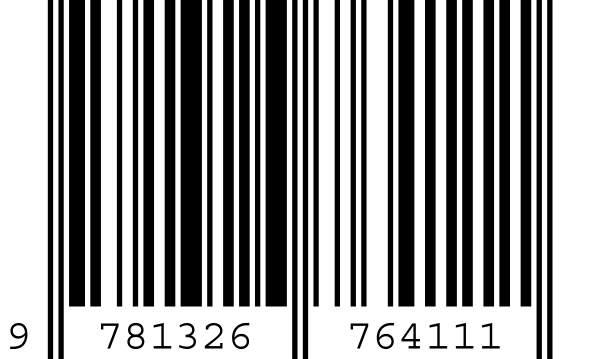
\includegraphics[width=4.7cm]{isbnbarcode}$
        	\end{minipage}
    	}
	}
}

\end{document}